\documentclass[ngerman]{scrartcl} 
%\KOMAoptions{fontsize=12pt, paper=a4}
%\KOMAoptions{DIV=11}
\usepackage[ngerman]{babel}
\def\nummer{0}
\author{Cornelius Heiming}	
\title{Versuch \nummer~:  Einf\"uhrungen und Vorversuch}
\date{29.04.2025}		
\usepackage{amsmath, amssymb, amsthm} 
\usepackage{geometry}
\usepackage[utf8]{inputenc}
\usepackage{enumerate}
\usepackage[shortlabels]{enumitem}

\usepackage{../pakete}
\usepackage{../aufgaben}

\addbibresource{../referenzen.bib}
\geometry{a4paper, left=3cm, right=3cm, top=3cm, bottom=3cm}

\newtheorem{theorem}{Satz}
\newtheorem{lemma}[theorem]{Lemma}
\newtheorem{korollar}{Korollar}[section]
\theoremstyle{definition}
\newtheorem{definition}[theorem]{Definition}
\newtheorem{beispiel}[theorem]{Beispiel}
\newtheorem{satz}[theorem]{Satz}

%\displaystyle \lim_{x \to \infty}

\begin{document}
	\maketitle
	\section{Einleitung}
		%TODO Was wird gemessen?
		%TODO Wodurch ist der Versuch motiviert, was ist das Ziel des Versuches
		In diesem Versuch wird der Oszillograph untersucht und insbesondere seine Anstiegszeit bestimmt. Dazu wird zunächst die Anstiegszeit eines Rechtecksignals ermittelt. Anschließend wird ein R-C-Filter mit einer Sinuswelle betrieben und daraus seine Grenzfrequenz bestimmt. 
	\section{Theorie}

		%TODO Kurze Darstellung der Physik für den Versuch, Grundlagen, Voraussetzungen
		%TODO Formeln, die in der Auswertung verwendet werden
		%TODO Prägnanz
		Beim Arbeiten mit Wechselstrom ist eine Visualisierung desselben notwendig. Diese erfolgt in der Regel mit einem Oszilloskop. Aufgrund von endlichen Ausbreitungsgeschwindigkeiten muss dieses, und auch der Signalgenerator eine positive Anstiegszeit haben. Entsprechend kann die Frequenz nicht beliebig sein, man spricht von der Frequenzbandbreite $B = f_\mathrm{grenz} = \frac{1}{2\pi \tau}$ mit $\tau = R \cdot C$, also modelliert als R-C Tiefpass. Die Bandbreite hängt gemäß der Aufgabe~\ref{voraufgabeD} mit der Anstiegszeit über die Formel $B \cdot \Delta t = \SI{0,35}{}$ zusammen.
	\section{Voraufgaben}
		\begin{voraufgabe}{Geben Sie für die Spannung $U(t) = U_0 \sin(\omega t)$ die Größen $U_\mathrm{SS}$, $U_\mathrm{S}$ und $U_\mathrm{eff}$ an.}
			Berechne zunächst $\langle \sin^2(\omega t) \rangle$:
			\begin{align*}
    \frac{2}{2T}\int_{-T}^T \sin^2(\omega t)\,dt 
    &= \frac{1}{2T}\int_{-T}^T \sin^2(\omega t)\,dt + \frac{1}{2T}\int_{-T}^T \sin^2(\omega t)\,dt \\
    &= \frac{1}{2T}\int_{-T}^T \sin^2(\omega t)\,dt + \frac{1}{2T}\int_{-T}^T \cos^2\left(\omega\left(t - \frac{\pi}{2\omega}\right)\right)\,dt \\
    &= \frac{1}{2T}\int_{-T}^T \sin^2(\omega t)\,dt + \frac{1}{2T}\int_{-T - \frac{\pi}{2\omega}}^{T - \frac{\pi}{2\omega}} \cos^2(\omega t)\,dt \\
    &= \frac{1}{2T}\int_{-T}^T \sin^2(\omega t)\,dt + \frac{1}{2T}\int_{-T}^{T} \cos^2(\omega t)\,dt \quad \text{(Periodizität von $\cos$)} \\
    &= \frac{1}{2T}\int_{-T}^T \left[\sin^2(\omega t) + \cos^2(\omega t)\right]\,dt \\
    &= \frac{1}{2T}\int_{-T}^T 1\,dt = 1 \\
    \Rightarrow \langle \sin^2(\omega t) \rangle &= \lim_{T \to \infty} \frac{1}{2T}\int_{-T}^T \sin^2(\omega t)\,dt = \frac{1}{2}
\end{align*}
Also gilt:
\begin{align*}
    U_\mathrm{SS} &= \max_t U(t) - \min_t U(t) = U_0 - (-U_0) = 2U_0 \\
    U_\mathrm{S} &= \max_t |U(t)| = U_0 \\
    U_\mathrm{eff} &= \sqrt{\langle U^2(t) \rangle} = U_0 \sqrt{\langle \sin^2(\omega t) \rangle} = U_0 \cdot \frac{1}{\sqrt{2}}
\end{align*}
		\end{voraufgabe}		
		\begin{voraufgabe}{Wie groß ist der Effektivwert eines symmetrischen Rechtecksignals mit $U_\mathrm{S} = \SI{10}{\volt} $?}			
			Ein Rechtecksignal kann mit 
			\begin{equation*}
				 U(t) = \begin{cases}
				U_\mathrm{S} & t \in \left[2n,2n+1\right) \text{ für } n \in \mathbb{Z}\\
				-U_\mathrm{S} & t \in \left[2n+1,2n+2\right) \mathrm{für} n \in \mathbb{Z}
			\end{cases}
			\end{equation*}
			beschrieben werden. Demnach gilt:
			\begin{align*}
				U_\mathrm{eff} &= \sqrt{\langle U^2(t) \rangle} \\
				&= \sqrt{\langle {(\pm U_\mathrm{S})}^2 \rangle}= U_{\mathrm{S}} \\
				&= \SI{10}{\volt}
			\end{align*}
		\end{voraufgabe}	
		\begin{voraufgabe}{Wie groß ist derAAA Innenwiderstand des Generatorausgangs?}
			\begin{align*}
				U_2-U_1 &= U_0\frac{R_2}{R_2+R_i}-U_0\frac{R_1}{R_1+R_i} \\
				&= U_0\frac{R_2(R_1+R_i)-R_1(R_2+R_i)}{(R_2+R_i)(R_1+R_i)} \\
				&= R_i\frac{U_0(R_2+R_i-R_1-R_i)}{(R_2+R_i)(R_1+R_i)} \\
				&= R_i\left(\frac{U_0(R_2+R_i)}{(R_2+R_i)(R_1+R_i)} - \frac{U_0(R_1+R_i)}{(R_2+R_i)(R_1+R_i)}\right) \\
				&= R_i\left(\frac{U_0}{R_1+R_i} - \frac{U_0}{R_2+R_i}\right) \\
				&= R_i(I_1 - I_2)
			\end{align*}
			Also gilt äquivalent:
			\begin{equation*}
				R_i = \frac{U_2-U_1}{I_1-I_2}
			\end{equation*}
			Nun soll mit den Angaben $U_\mathrm{SS} = \SI{20}{\volt_\mathrm{SS}}$ bei $I_1=\SI{0}{\ampere}$ und $U_\mathrm{SS} = \SI{20}{\volt_\mathrm{SS}}$ bei $\SI{50}{\ohm}$ Last der Innenwiderstand berechnet werden. Die Amplitude beträgt die Hälfte des Spitze-Spitzewertes, d.h. $U_1 = \SI{10}{\volt_\mathrm{S}}$, $I_1 = \SI{0}{\ampere}$ sowie $U_2 = \SI{5}{\volt_\mathrm{S}}$, $I_2 = \frac{\SI{5}{\volt_\mathrm{S}}}{\SI{50}{\ohm}} = \SI{0,1}{\ampere}$:
			\begin{align*}
			    R_i &= \frac{\SI{5}{\volt}-\SI{10}{\volt}}{\SI{0}{\ampere}-\SI{0,1}{\ampere}} \\
    			&= \SI{50}{\ohm}
			\end{align*}
		\end{voraufgabe}
		\stepcounter{voraufgabe}
		\begin{voraufgabe}{Zeigen Sie, dass für einen einfachen Tiefpass (exponentiell ansteigende Flanke) näherungsweise die Formel $B \cdot \Delta t = \SI{0,35}{}$ gilt.}
		\label{voraufgabeD}
		Für einen Tiefpass gilt die Formel: 
		\begin{align*}
   			 U(t) = U_0 (1-\exp(-\frac{t}{\tau}))
		\end{align*}
		Seien $t_1$ und $t_2=t_1+\Delta t$ die Zeitpunkte, zu denen $\SI{10}{\percent}$ und $\SI{90}{\percent}$ von $U_0$ erreicht sind. Dann folgt:
		\begin{align*}
    		\SI{0,1}{} &= \exp(-\frac{t_1+\Delta t}{\tau}) \notag \\
    		&=\underbrace{\exp(-\frac{t_1}{\tau})}_{\SI{0,9}{}}\cdot\exp(-\frac{\Delta t}{\tau}) \notag \\
    		\Leftrightarrow \ln(9) &= \frac{\Delta t}{\tau} \notag \\
    		&= 2\pi B \Delta t \notag \\
    		\Leftrightarrow B \Delta t &= \frac{\ln(9)}{2\pi} \approx \SI{0,35}{}
    		\label{eq:035}
		\end{align*}

\end{voraufgabe}
		%TODO Voraufgaben
% === Aufbau, Durchführung, Messwerte und Auswertung ===
	\section{Versuchsaufbau, -durchführung, Messwerte und Auswertung}
		\begin{aufgabe}{Bestimmung der Anstiegszeit des Oszillographen}
			\aufbau
			\begin{figure}[H]
				\centering
				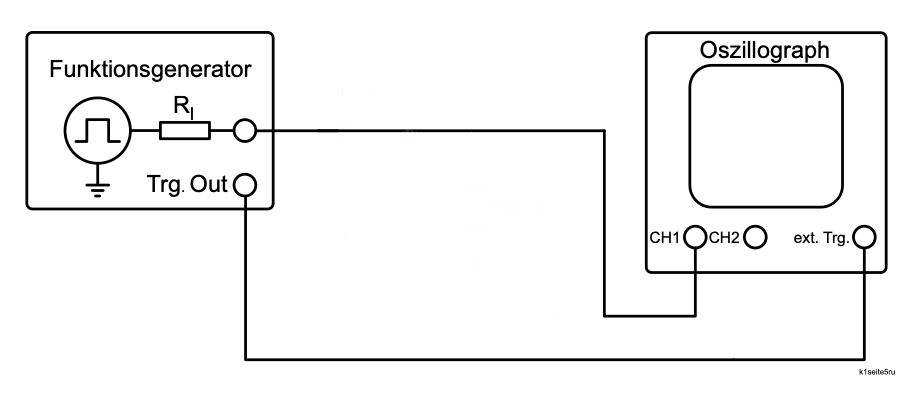
\includegraphics[width=0.8\textwidth]{figs/Aufbau_0_1_Oszilloskop.png}
				\caption{Schaltplan Funktionsgenerator und Oszilloskop~\cite{anleitung}}
				\label{fig:aufbau_0_1_oszilloskop.png}
			\end{figure}
			\begin{enumerate}[(a)]
				\item In dieser Aufgabe soll der Oszillograph untersucht werden. Dafür wird der Generatorausgang mit dem CH1 Eingang des Oszilloskops mittels eines Koaxialkabels verbunden. Nach dem Triggern können verschiedene Oszillogramme beobachtet werden.
				\item Danach wird ein Rechtecksignal mit einer Frequenz von $\SI{2}{\mega\hertz}$ und einer Amplitude von beispielsweise $\SI{1}{\volt}$ eingestellt. Die Anstiegszeit $\Delta t_\mathrm{gemessen}$ wird bestimmt, indem die Zeitdifferenz zwischen dem Zeitpunkt, an dem $U(t)$ den Wert $0.1 U_0$ erreicht, und dem Zeitpunkt, an dem $U(t)$ den Wert $0.9 U_0$ erreicht, gemessen wird.
				\item Zuletzt wird der Generatorausgang mit einem R-C-Filter verbunden. Es soll eine Zeitkonstante von $\tau = \mathcal{O}(\SI{10}{\micro\second} \text{ bis } \SI{100}{\micro\second})$ realisiert werden, also können bspw. $R = \SI{1}{\kilo\ohm}$ und $C = \SI{10}{\micro\farad}$ gewählt werden. Der R-C-Filter wird erneut mit dem CH1-Eingang des Oszilloskops verbunden. Der Generator wird auf ein Sinus-Signal mit 10 verschiedenen Frequenzen eingestellt. Dabei wird sich jeweils die Amplitude am Signalgenerator notiert.
			\end{enumerate}
			\MesswUndAusw
			\begin{unteraufgabe}
				\begin{figure}[H]
					\centering
					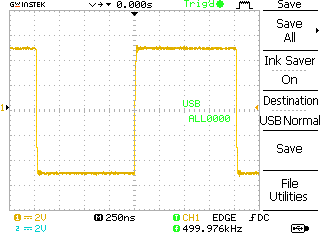
\includegraphics[width=0.8\textwidth]{MesswerteVersuch0/A0000DS.png}
					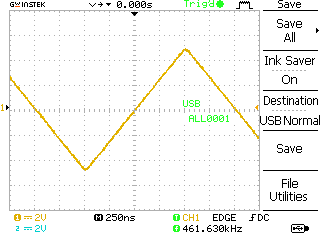
\includegraphics[width=0.8\textwidth]{MesswerteVersuch0/A0001DS.png}
					\caption{Oben: Rechtecksignal, unten: Dreieckssignal}
					\label{fig:A0000DS,1}
				\end{figure}
				\begin{figure}[H]
					\centering
					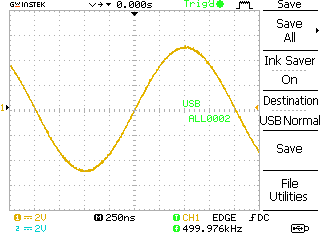
\includegraphics[width=0.8\textwidth]{MesswerteVersuch0/A0002DS.png}
					\caption{Sinussignal}
					\label{fig:A0002DS}
				\end{figure}
			\end{unteraufgabe}
			\begin{unteraufgabe}
				\begin{figure}[H]
					\centering
					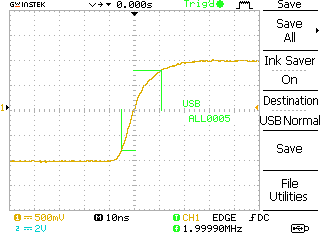
\includegraphics[width=0.8\textwidth]{MesswerteVersuch0/A0005DS.png}
					\caption{Rechteckssignalanstieg (detailliert)}
					\label{fig:A0005DS}
				\end{figure}
				Aus der Grafik \ref{fig:A0005DS} kann die Anstiegszeit $\Delta t_\mathrm{gemessen}$ abgelesen werden. Dafür wurden die $10\%$ und $90\%$ markiert und damit die Zeitpunkte ermittelt, an denen die Spannung $U(t)$ den Wert $0.1 U_0$ und $0.9 U_0$ erreicht. Die Anstiegszeit $\Delta t_\mathrm{gemessen}$ beträgt dann $\SI{16}{\nano\second}$ (Genau $8$ Einheiten der Skala, die je $\frac{1}{5}$ von $\SI{10}{\nano\second}$ sind). Der Messfehler beträgt $4$ Pixel, also $\Delta(\Delta t_\mathrm{gemessen}) =  \SI{1}{\nano\second}$. Der Betriebsanleitung des Oszilloskops \cite{oszibedienungsanleitung} zufolge beträgt die Bandbreite des Oszilloskops $B = \SI{50}{\mega\hertz}$. Daraus folgt mit der Formel $B \cdot \Delta t = \SI{0.35}{}$ (siehe Voraufgabe~\ref{voraufgabeD}) die Anstiegszeit:
				\begin{align*}
					\Delta t_\mathrm{Oszi} = \frac{0.35}{\SI{50}{\mega\hertz}} = \SI{7}{\nano\second}
				\end{align*}
				Für die Anstiegszeit des Signals $\Delta t_\mathrm{Signal}$ gilt nach der Anleitung\cite{anleitung} die Näherung:
				\begin{align*}
					(\Delta t_\mathrm{Signal})^2 &= (\Delta t_\mathrm{Oszi})^2 - (\Delta t_\mathrm{gemessen})^2 \\
					\Delta t_\mathrm{Signal} &= \sqrt{(\Delta t_\mathrm{Oszi})^2 - (\Delta t_\mathrm{gemessen})^2} \\
					&= \sqrt{(\SI{16}{\nano\second})^2 - (\SI{7}{\nano\second})^2} \approx \SI{14.39}{\nano\second}
				\end{align*}
				Mittels Gaußscher Fehlerfortpflanzung ergibt sich:
				\begin{align*}
					\Delta(\Delta t_\mathrm{Signal}) &= \frac{2 t_\mathrm{gemessen}}{\sqrt{(\Delta t_\mathrm{gemessen})^2 - (\Delta t_\mathrm{Oszi})^2}} \cdot \Delta(\Delta t_\mathrm{gemessen}) \\
					&= \frac{2 \SI{16}{\nano\second}}{\sqrt{(\SI{16}{\nano\second})^2 - (\SI{7}{\nano\second})^2}} \cdot \SI{1}{\nano\second} \\
					&\approx \SI{2.3}{\nano\second}
				\end{align*}
				Also ergibt sich für die Anstiegszeit des Signals:
				\begin{align*}
					\Delta t_\mathrm{Signal} &= \SI{14.4}{\nano\second} \pm \SI{2.3}{\nano\second}
				\end{align*}
			\end{unteraufgabe}
			\begin{unteraufgabe}
				\begin{figure}[H]
					\centering
					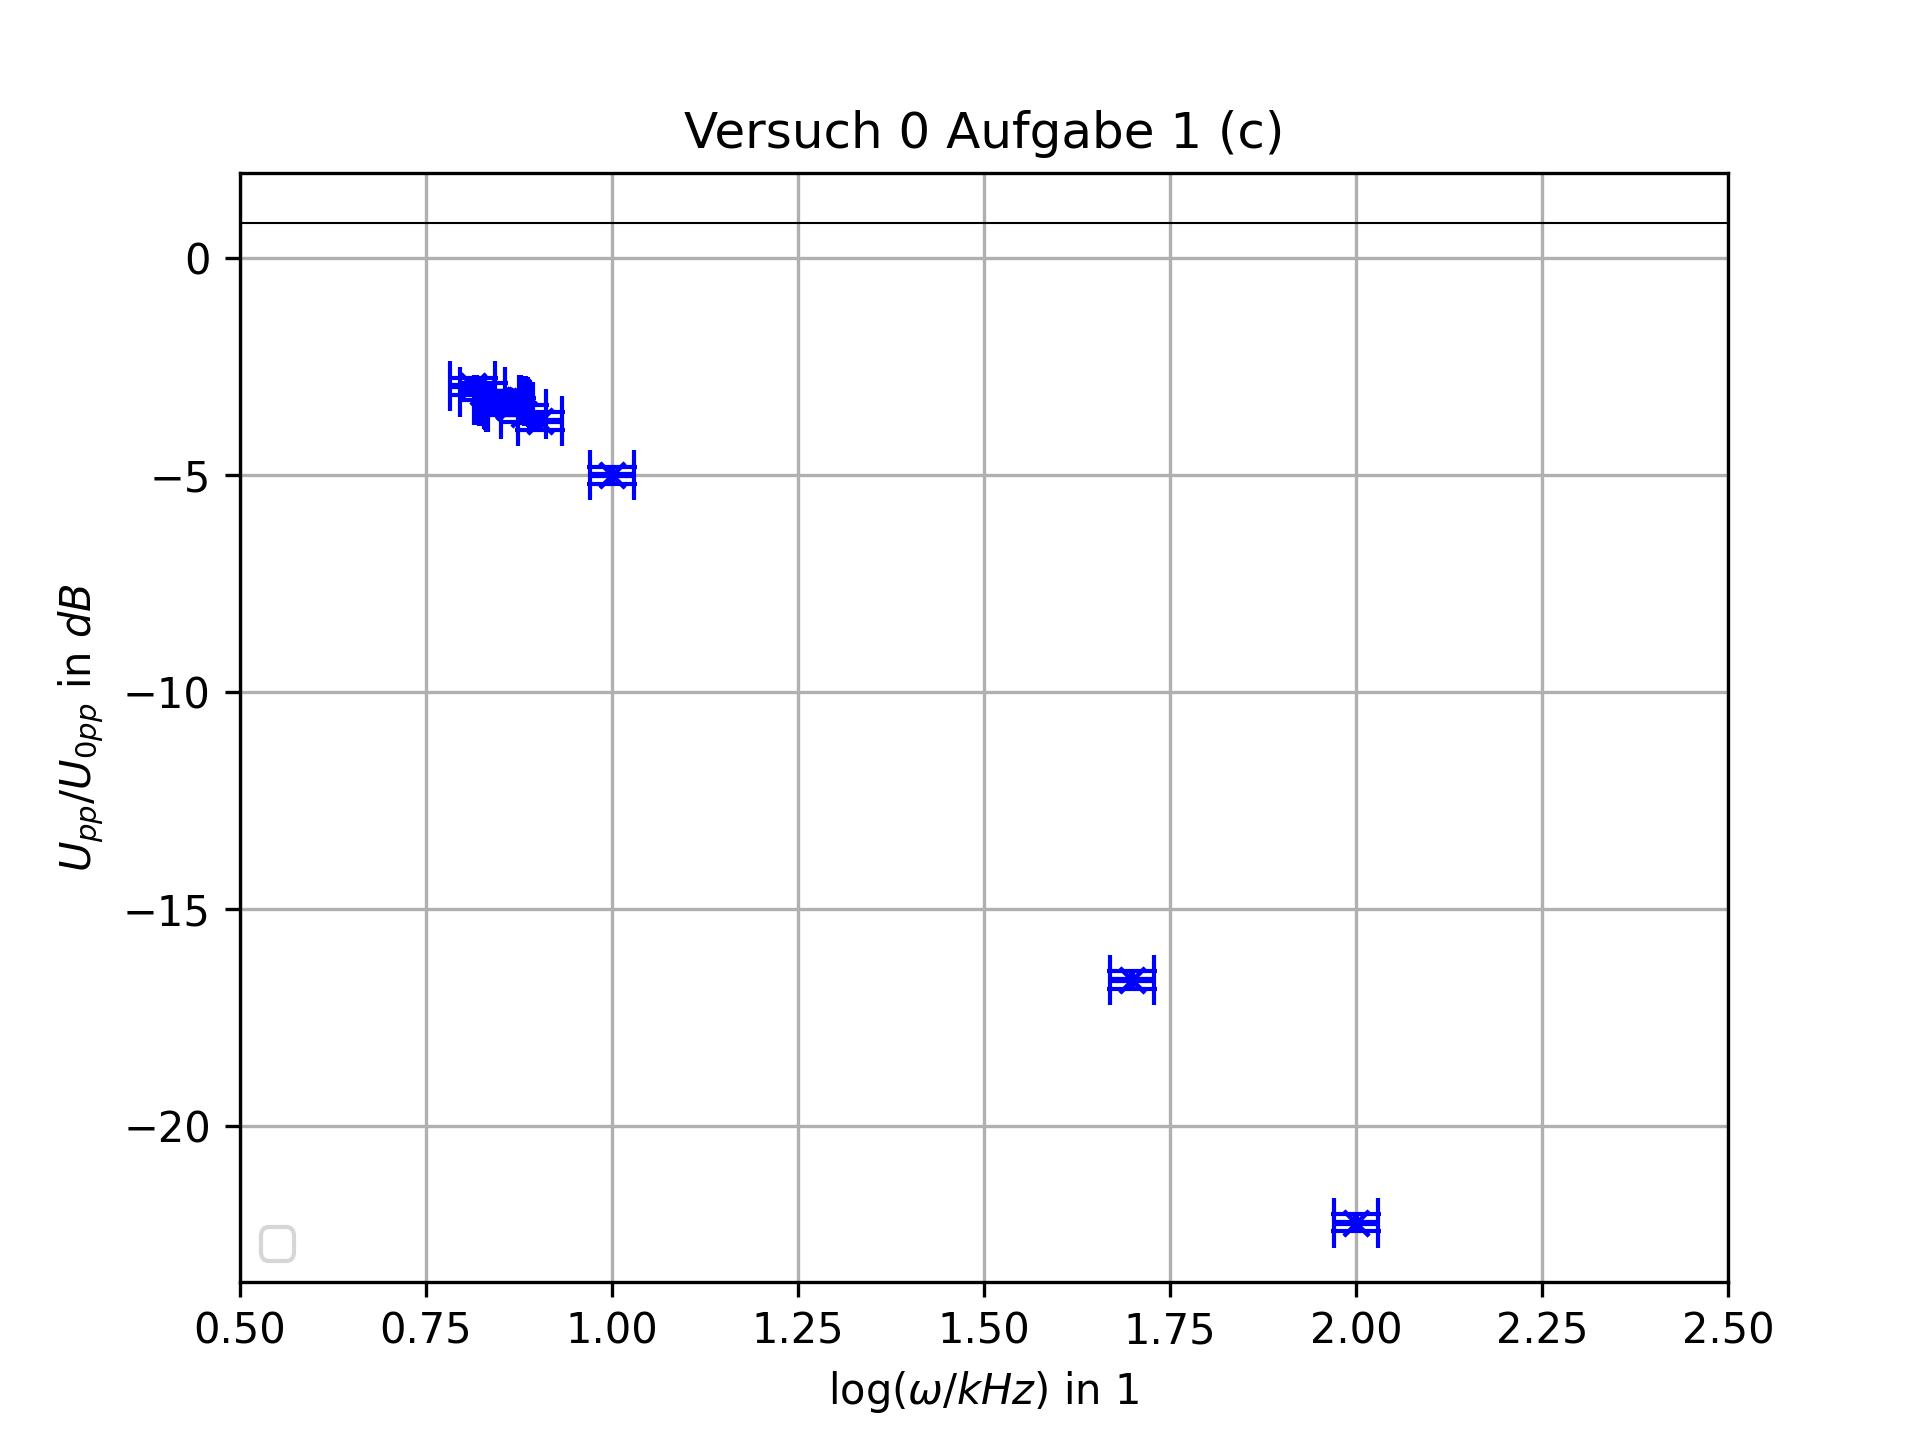
\includegraphics[width=0.8\textwidth]{pythonAuswertungen/Versuch 0 Aufgabe 1 (c)_plot.jpg}
					\caption{Dämpfungsplot}
					\label{0_1_(c)_Dämpfung}
				\end{figure}
				%TODO: c) Tabelle machen, auswerten.
			\end{unteraufgabe}

		\end{aufgabe}
			%TODO Aufbau/Schaltskizze (beschrieben in wenigen Worten)
			%TODO Versuchsdurchführung: Messgrößen, unabh. Parameter, Messmethode, Einheiten, Genauigkeit, wie oft
			%TODO Abgezeichnetes Messprotokoll vorhanden?
			%TODO Auswertung (in Worten & Formeln)
			%TODO Formeln symbolisch und numerisch
			%TODO Runden
			%TODO Grafiken & Diagramme: Überschrift, Messwerte mit Fehlerbalken, (nur) gefittete Kurven, Achsenbeschriftung
			%TODO Fehlerrechnung und -diskussion
			%TODO Jede Tabelle eine Formel
		\section{Endresultat}
			%TODO Vollständiger Satz
		\section{Ergebnisdiskussion/Plausibilitätskontrolle}
			
			%TODO Messergebnisse bewerten und evtl. mit Literaturwerten vergleichen
			%TODO Untersuchung Fehlerquellen (statistisch, systematisch, blödsinnig)
		%\printbibliography
\end{document}
